\documentclass[a4paper, 12pt]{article}
\usepackage[T1]{fontenc}
\usepackage[utf8]{inputenc}
\usepackage{graphicx}
\usepackage{hyperref}
\usepackage{url}

\hypersetup{
    pdfborder={0 0 0}
}

\newcounter{tc}

\begin{document}

\newcommand{\code}[1]{
    \texttt{#1}
}

\newcommand{\testx}[7]{
	\stepcounter{tc}
	\subsection{Test \thetc: #1} % (fold)

	% subsubsection test_1 (end)
	\begin{tabular}{l p{0.7\textwidth}}
    \hline
    \textbf{Test Case Identifier} & \thetc\\
    \hline
    \textbf{Test Item(s)} & \code{#2} $\rightarrow$ \code{#3}\\
    \hline
    \textbf{Input Specification} & #4\\
    \hline
    \textbf{Output Specification} & #5\\
    \hline
    \textbf{Environmental Needs} & #6\\
    \hline
    \textbf{Test Description} & #7\\
    \hline
	\end{tabular}
}

\title{Integration Test Plan Document}

\author{M. Albanese, M. Bianchi, A. Carlucci}

\maketitle
\newpage{}
\tableofcontents{}

\newpage{}

\section{Introduction}
% \subsection{Revision History}
% \label{sub:revision_history}

\subsection{Purpose}
\label{sub:purpose}
The purpose of this document, the \textbf{Integration Test Plan Document} (ITPD), is to describe how integration tests are to be performed.

The tests that will be described here will mainly focus on the flow of information between different modules rather than on the modules themselves.
In particular, it describes the adopted methodologies, the sets of all tests to be performed, the tools that will be used during the whole process.

\subsection{Scope} % (fold)
\label{sub:scope}
The system will be an optimization of a pre-existing, non-software solution for renting taxis already in use in the city. The new system will let users to rent or reserve a taxi through a mobile or a web application and will also let taxi drivers to take care of the users' requests in a more simple and effective way. In addition to a better user interface, the new system will focus on a smarter organization of the vehicles deployed in each city zone, resulting in a more efficient service for the citizens.

% subsection scope (end)

\newpage
\subsection{List of definitions and abbreviations}
\label{sub:list_of_definitions_and_abbreviations}

\begin{description}
    \item[JUnit] The tool used for unit testing. See Section~\ref{sub:tools_and_test_equipment_required} for more information.
    \item[Mockito] A mocking framework used in conjuction with JUnit.
    \item[Arquillian] The tool used for the actual integration testing. See Section~\ref{sub:tools_and_test_equipment_required} for more information.
    \item[RASD] Requirements \& Analysis Specification Document
    \item[DD] Design Document
    \item[ITPD] Integration Test Plan Document
    \item[DBMS] Database Management System
    %\item[]
\end{description}

\newpage
\section{Integration Strategy}
\label{sec:integration_strategy}

\subsection{Entry Criteria}
\label{sub:entry_criteria}
Several entry criteria must be met before Integration Testing phase.

The whole architecture must be designed according to the contents of the \textbf{Design Document}, to be written along with this one.
Following this phase, each component that will be integrated must be - of course - coded.

After development phase, each module must successfully pass a thorough \textbf{unit testing}, which guarantees the absence of critical bugs in the codebase. As stated in Section~\ref{sub:tools_and_test_equipment_required}, JUnit will be the privileged tool for this phase.

Along with unit testing, code inspection is done, via both manual and automated work; all these devices will lead to well-formed and robust modules, ready to be composed together.

\subsection{Elements to be integrated}
\label{sub:elements_to_be_integrated}

\begin{figure}[htb]
    \centering
    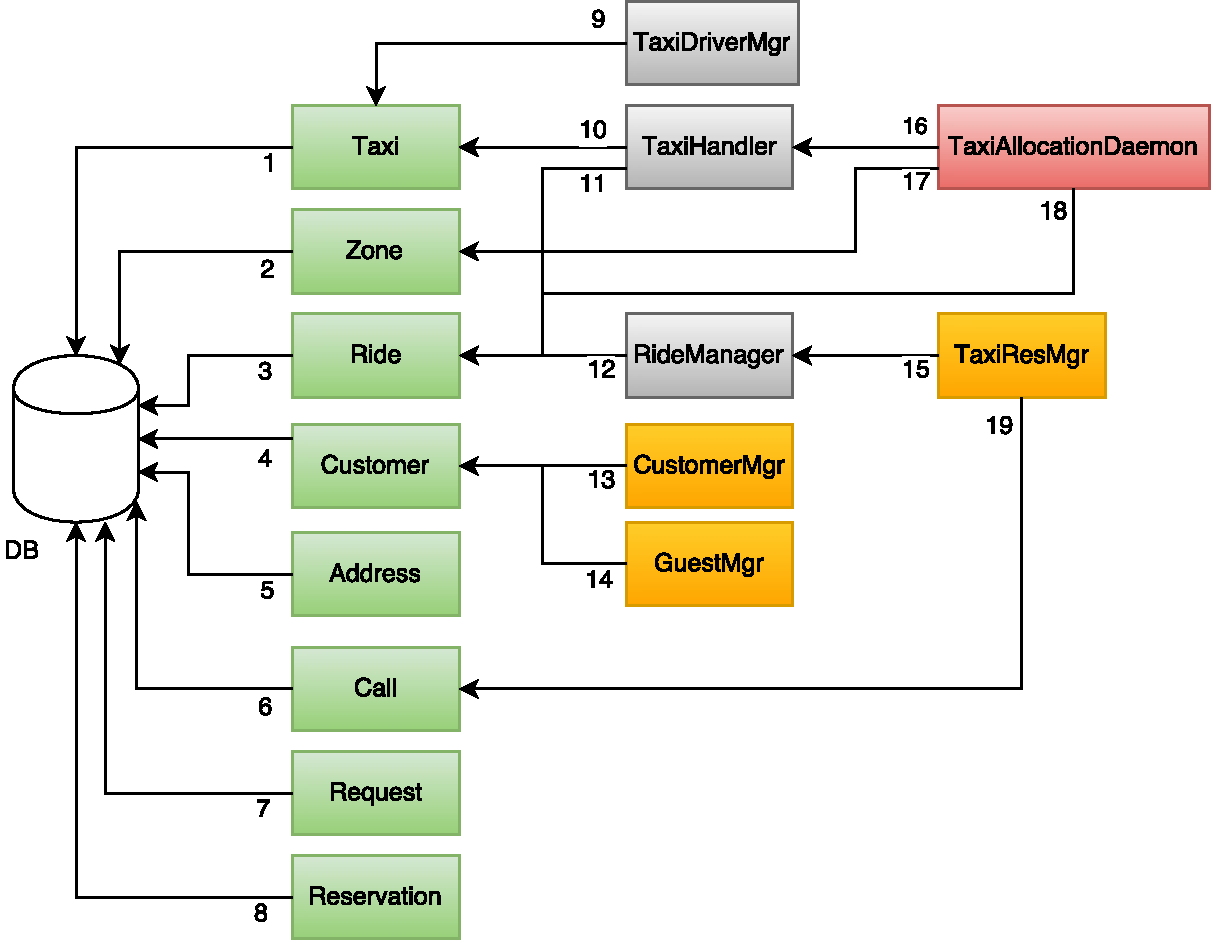
\includegraphics[width=1.2\textwidth]{img/elements.pdf}
    \label{fig:testplan}
\end{figure}

\begin{table}
    \centering
    \begin{tabular}{| l | l | p{0.35\textwidth} | p{0.3\textwidth} |}
    \hline
    \textbf{ID} & \textbf{Component} & \textbf{Subsystem} \\
    \hline
    A & DAOs & DataLayer \\
    \hline
    1 & GuestManager & ClientMgr\\
    \hline
    2 & Customer & DataLayer\\
    \hline
    3 & CustomerManager & ClientMgr\\
    \hline
    4 & Address & DataLayer\\
    \hline
    5 & Call & DataLayer\\
    \hline
    6 & Reservation & DataLayer\\
    \hline
    7 & Request & DataLayer\\
    \hline
    8 & Ride & DataLayer\\
    \hline
    9 & TaxiResMgrManager & TaxiResMgr\\
    \hline
    10 & RideManager & TaxiResMgr\\
    \hline
    11 & TaxiAllocationDaemon & TaxiAllocationMgr\\
    \hline
    12 & Zone & DataLayer\\
    \hline
    13 & TaxiHandler & TaxiAllocationMgr\\
    \hline
    14 & Taxi & DataLayer\\
    \hline
    15 & TaxiDriverManager & TaxiDriverMgr\\
    \hline
    \end{tabular}
    \caption{List of all components to be integrated. The list of all Data Access Objects is omitted for simplicity.}
    \label{tab:components}
\end{table}

\subsection{Integration Testing Strategy}
\label{sub:integration_testing_strategy}
The strategy that will be adopted is the so-called \textbf{bottom-up} approach.

An incremental approach is fundamental, in order to prevent all shortcomings that are typical to \emph{Big Bang approach} (you have to wait until all modules are complete, localizing the faulty components can be difficult, some interfaces could be missed easily during testing...).

We decided to choose bottom-up over top-down because there are many components at the lower levels (see Figure~\ref{fig:testplan}); this means that only few drivers, if any, are needed.

\subsection{Sequence of Component/Function Integration}
\label{sub:sequence_of_component_function_integration}

\subsubsection{Software Integration Sequence}
\label{ssub:software_integration_sequence}
\begin{table}
    \centering
    \begin{tabular}{| l | l | l | l | l |}
    \hline
    \textbf{Test ID} & \textbf{Component 1} & \textbf{Subsystem 1} & \textbf{Component 2} & \textbf{Subsystem 2} \\
    \hline
    1 & Taxi & TaxiDriver & DBMS & DBMS \\
    \hline
    2 & Zone & TaxiAllocation & DBMS & DBMS \\
    \hline
    3 & Ride & TaxiReservation & DBMS & DBMS \\
    \hline
    4 & Customer & Client & DBMS & DBMS \\
    \hline
    5 & Address & TaxiReservation & DBMS & DBMS \\
    \hline
    6 & Call & TaxiReservation & DBMS & DBMS \\
    \hline
    7 & Request & TaxiReservation & DBMS & DBMS \\
    \hline
    8 & Reservation & TaxiReservation & DBMS & DBMS \\
    \hline
    9 & TaxiDriverMgr & TaxiDriver & Taxi & TaxiDriver \\
    \hline
    10 & TaxiHandler & TaxiAllocation & Taxi & TaxiDriver \\
    \hline
    11 & TaxiHandler & TaxiAllocation & Ride & TaxiReservation \\
    \hline
    12 & RideManager & TaxiReservation & Ride & TaxiReservation \\
    \hline
    13 & CustomerManager & Client & Customer & Client \\
    \hline
    14 & GuestManager & Client & Customer & Client \\
    \hline
    15 & TaxiResManager & TaxiReservation & RideManager & TaxiReservation \\
    \hline
    16 & TaxiAllocationDaemon & TaxiAllocation & TaxiHandler & TaxiAllocation \\
    \hline
    17 & TaxiAllocationDaemon & TaxiAllocation & Zone & TaxiAllocation \\
    \hline
    18 & TaxiAllocationDaemon & TaxiAllocation & Ride & TaxiReservation \\
    \hline
    19 & TaxiResManager & TaxiReservation & Call & TaxiReservation \\
    \hline
    \end{tabular}
    \caption{List of all components to be integrated}
    \label{tab:components-integration}
\end{table}

\subsubsection{Subsystem Integration Sequence}
\label{ssub:subsystem_integration_sequence}

QUI SUI SUBSYSTEM
\begin{table}
    \centering
    \begin{tabular}{| l | l | l |}
        \hline
        \textbf{N.} & \textbf{Subsystem} & \textbf{Integrates with} \\
        \hline
        1 & Client & DBMS \\
        2 & TaxiRes & DBMS \\
        3 & TaxiAllocation & DBMS \\
        4 & Client & TaxiReservation \\
        5 & TaxiAllocation & TaxiReservation \\
        6 & TaxiDriver & TaxiAllocation \\
        7 & Mobile App & TaxiDriver \\
        \hline
    \end{tabular}
    \caption{Integration order of the subsystems.}
    \label{tab:subsystem-integration}
\end{table}

QUI ANDRA TESTO SUI TIER

\begin{table}
    \centering
    \begin{tabular}{| l | l | l |}
        \hline
        \textbf{N.} & \textbf{Subsystem} & \textbf{Integrates with} \\
        \hline
        1 & Core (Back-end) & DBMS \\
        2 & Taxi Driver mobile application & Core \\
        3 & Mobile UI & Core \\
        4 & Web UI & Core \\
        \hline
    \end{tabular}
    \caption{Integration order of the tier composing the whole architecture}
    \label{tab:tier-integration}
\end{table}

\newpage
\section{Individual Steps and Test Description}
\label{sub:individual_steps_and_test_description}

% === DB ===
\testx{Taxi - Access to DB}{Taxi}{DBMS}{Frequent queries on table Taxi}{The corresponding tuples to the query}{DB working}{Verify that all entities in the DB are correctly mapped through JavaBeans}

\testx{Zone - Access to DB}{Zone}{DBMS}{Frequent queries on table Zone}{The corresponding tuples to the query}{DB working}{Verify that all entities in the DB are correctly mapped through JavaBeans}

\testx{Ride - Access to DB}{Ride}{DBMS}{Frequent queries on table Ride}{The corresponding tuples to the query}{DB working}{Verify that all entities in the DB are correctly mapped through JavaBeans}

\testx{Customer - Access to DB}{Customer}{DBMS}{Frequent queries on table Customer}{The corresponding tuples to the query}{DB working}{Verify that all entities in the DB are correctly mapped through JavaBeans}

\testx{Address - Access to DB}{Address}{DBMS}{Frequent queries on table Address}{The corresponding tuples to the query}{DB working}{Verify that all entities in the DB are correctly mapped through JavaBeans}

\testx{Call - Access to DB}{Call}{DBMS}{Frequent queries on table Call}{The corresponding tuples to the query}{DB working}{Verify that all entities in the DB are correctly mapped through JavaBeans}

\testx{Request - Access to DB}{Request}{DBMS}{Frequent queries on table Request}{The corresponding tuples to the query}{DB working}{Verify that all entities in the DB are correctly mapped through JavaBeans}

\testx{Reservation - Access to DB}{Reservation}{DBMS}{Frequent queries on table Reservation}{The corresponding tuples to the query}{DB working}{Verify that all entities in the DB are correctly mapped through JavaBeans}

% === OTHERS ===
\testx{TaxiDriverManager - Update Taxi entity}{TaxiDriverManager}{Taxi}{Update information on position and status of the taxi}{Taxi has modified data}{Working Glassfish Server}{The purpose of this test is to verify that all the information are correctly updated on the server}

\testx{TaxiHandler - Taxi assignment to a ride}{TaxiHandler}{Taxi}{New ride available}{Ride assigned to taxi}{Working Glassfish Server}{Verify that a new ride is properly assigned to a taxi in the correct zone}

\testx{TaxiHandler - Ride completion with a taxi}{TaxiHandler}{Ride}{New ride on schedule}{Taxi assigned to the specified ride}{Working Glassfish Server}{Verify that a taxi is correctly assigned to the ride}

\testx{RideManager - Operations on rides}{RideManager}{Ride}{ Some ride specification needs to be changed. }{ The corresponding ride is changed. }{ Working Glassfish server, Working Database server }{ Verify that RideManager is working correctly }

\testx{CustomerManager - Customer Services}{CustomerManager}{Customer}{There are some pending operations initiated by users.}{For each operation, every involved user entity must be updated correctly, according to the specified operation.}{Working Glassfish Server, Working Database server}{Verify that CustomerManager is working properly.}

\testx{GuestManager - Guest Services}{GuestManager}{Customer}{There are some pending operations initiated by customers.}{ Every operation must be executed correctly, according to the user level (unregistered!)}{Working Glassfish Server, Working Database server}{Assert that every guest operation is working properly.}

\testx{TaxiResManager - Check existing rides}{TaxiResManager}{RideManager}{
Call to existRide()
}{Return value must be chosen according to the existance of this ride}{Working Glassfish Server, Working Database server}{Check that RideManager will give back valid results.}

\testx{TaxiAllocationDaemon - Creation of a handler for an incoming ride}{TaxiAllocationDaemon}{TaxiHandler}{Ride to be handled}{Association between a ride and a taxi}{Working Glassfish Server, Working Database server}{Verify that an handler is created for every incoming ride}

\testx{TaxiAllocationDaemon - Avialable taxis in zones}{TaxiAllocationDaemon}{Zone}{Queue related to a zone}{Number of available taxi for a zone}{Working Glassfish Server, Working Database server}{The purpose of the test is to check that the number of available taxi in every zone is equal to each corresponding zone queue}

\testx{TaxiAllocationDaemon - Retrieve ride information}{TaxiAllocationDaemon}{Ride}{Ride on schedule}{Ride used in the creation of  new TaxiHandler}{Working Glassfish Server, Working Database server}{The purpose is to check that the proper information are correctly retrived and used for the creation of a new TaxiHandler}

\testx{TaxiResManager - Creation of a call}{TaxiResManager}{Call}{Information provided by the user}{New Call entity}{Working Glassfish Server, Working Database server}{Verify that a new call is correctly added}

\newpage
\section{Tools and Test Equipment Required}
\label{sub:tools_and_test_equipment_required}

\begin{description}
    \item[JUnit] JUnit is a simple framework to write repeatable tests. Each test is done on a single unit, usually composed of one public class. Tests can also be grouped in Suites for multiple instances at once.

    Since complex environments must be described within this project (for example, the interaction between \code{TaxiHandler} and \code{Taxi} or all interactions between a module and the DBMS), a mock framework is necessary. Among several and similar products(JMock, EasyMock, Powermock...), we decided to use \textbf{Mockito} for its simplicity and clearness.

    These tools are used \emph{before} Integration Testing happens (described throughout this document).

    \item[Arquillian] Arquillian is an integration testing framework for business objects that are executed inside a container or that interact with the container as a client. \\
\\
Arquillian combines a unit testing framework (JUnit), and one or more supported target containers (Java EE container, servlet container, etc) to provide a simple, flexible and pluggable integration testing environment. \\ \\ 
Arquillian strives to make integration testing no more complicated than basic unit testing, so we decided to use Arquillian as our integration testing framework for its semplicity.


\end{description}

\newpage
\section{Program Stubs and Test Data Required}
\label{sub:program_stubs_and_test_data_required}

\appendix

\clearpage
\addcontentsline{toc}{section}{References}

\begin{thebibliography}{9}
\bibitem{bib:assignment}
    Prof. Di Nitto - \emph{Assignment 4 - Integration Test Plan}

\bibitem{bib:spingrid}
    AA.VV. - \emph{SpinGrid - Integration Test Plan Example}

\bibitem{rasd}
        Albanese Michele, Bianchi Mattia, Carlucci Alain - \emph{myTaxiService: Requirements Analysis and Specification Document}

\bibitem{dd}
        Albanese Michele, Bianchi Mattia, Carlucci Alain - \emph{myTaxiService: Design Document}

\bibitem{Arquillian}
        AA.VV. - \emph{Arquillian Reference Guide} {\small(\url{https://docs.jboss.org/author/display/ARQ/Reference+Guide?_sscc=t})}

\bibitem{Mockito}
        AA.VV. - \emph{Mockito Reference Guide} {\small(\url{http://site.mockito.org/mockito/docs/current/org/mockito/Mockito.html})}
\end{thebibliography}

\vfill

% \section*{Hours spent}
% \begin{figure}[htb]
%     \centering
%     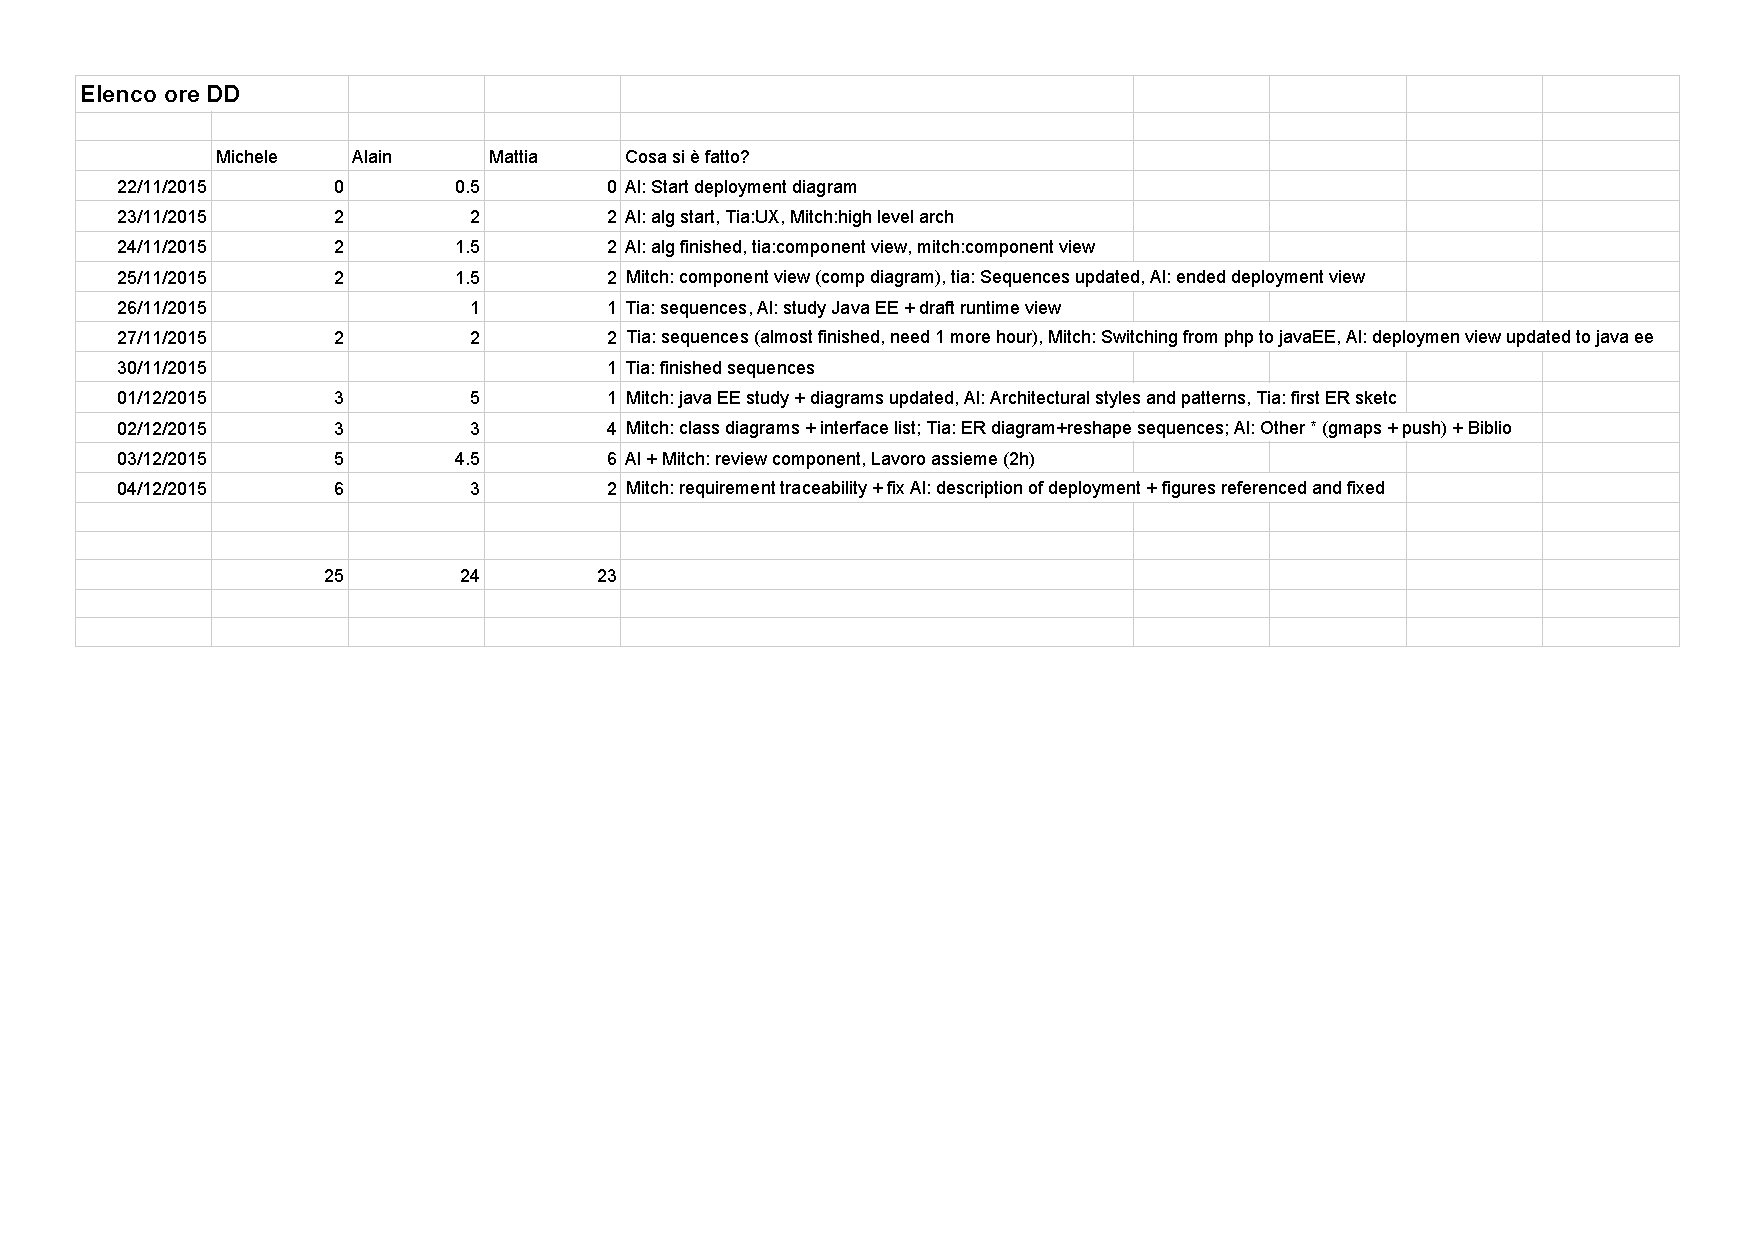
\includegraphics[width=1.2\textwidth]{img/hours.pdf}
%     \label{fig:hours}
% \end{figure}

\end{document}
